\chapter{Measuring and designing repository retrieval}\label{measuring-and-designing-repository-retrieval}

In my own benchmark built from tasks across 73 repositories, two instruments disagreed about the same retrieval tool. \href{mailto:Precision@10}{\nolinkurl{Precision@10}}, the proportion of the first ten results judged relevant, rose from 0.095 to 0.313. \textbf{\href{mailto:Recall@k}{\nolinkurl{Recall@k}}}, the fraction of judged needed items found among the first \(k\) results, rose at \(k=10\) from 0.120 to 0.272. The fraction of tasks for which the needed file appeared rose from 0.33 to 0.56. The paired end-to-end reward across 370 tasks moved by only +0.0349, with a bootstrap 95\% confidence interval of {[}+0.0130, +0.0579{]}, n = 370.

This bootstrap treated all 370 task-level deltas as independent observations. The tasks were drawn from 73 repositories and grouped into 20 suites, and the resampling reflected neither structure. The reported interval therefore likely understates the uncertainty and should not be read as a bound on it.

Chapter 1's rule about choosing the resampling unit applies directly here, but promoting the unit to the repository or to the suite is not sufficient on its own. Repositories and suites are two groupings over the same tasks. Whether they are nested or crossed determines whether one clustered unit is adequate or the analysis needs a hierarchical or multiway resampling procedure.

The retrieval measurements showed that the tool had become substantially better at putting relevant repository evidence in front of the agent. The final score showed that the system as a whole had changed little. Each scoring procedure estimated a different event.

This disagreement changed the engineering question. If I had kept only the final reward, I would have treated the retriever as a weak intervention and looked elsewhere. The stage measurements showed that retrieval had improved while much of the added evidence failed to become correct edits. The next investigation therefore belonged downstream, in context assembly, evidence use, generation, or verification.

The reverse pattern would have required a different explanation. An end-to-end gain without a retrieval gain could have come from a model change, a prompt difference, or some other uncontrolled part of the path.

Repository retrieval sits inside a causal chain. A task becomes one or more queries. Each query searches an index. Ranked results enter a context budget. A model interprets that context, and an execution and verification process turns the model's output into a scored result. A pass rate records the state at the end of the chain, and it cannot identify which transition produced that state.

\section{Score retrieval and generation separately}\label{score-retrieval-and-generation-separately}

Chapter 2 used ablations to isolate a component by removing it while holding the surrounding system fixed. Stage-level scoring applies the same attribution discipline within a run. I measure whether the retriever surfaced the evidence the task required, where that evidence appeared, whether it survived the context cutoff, and whether the generator used it. I report those measurements beside the final completion score, because each describes a different condition for success.

The first condition is availability. The relevant file, symbol, documentation block, or prior decision must exist in the searchable corpus and in its index. A retriever cannot return a file omitted by an indexing rule, a generated source tree excluded as noise, or a recently changed document still waiting for an asynchronous update. Treating these as ranking failures sends the investigation toward query tuning when the actual defect is corpus coverage or freshness.

The second condition is retrieval. Given an indexed target, the query must bring it into the returned set. The third is placement, because a relevant item can appear too low in the list to survive a fixed depth or token budget.

The fourth condition is contextual sufficiency. A method signature may be relevant but insufficient when the implementation, callers, or type definition determine the edit. The fifth is use. The model may receive adequate evidence and still ignore it, misread it, or produce an edit that fails for an unrelated reason.

An end-to-end failure is compatible with failure at any one of these conditions, and also with several at once. A tool can find the right method at position twelve, the context builder can keep ten results, and the generator can then invent an interface from the remaining snippets. The final failure does not reveal whether query formation, ranking, truncation, or generation should change. The trace does, but only when the evaluation has recorded the boundaries between those stages.

\begin{figure}
\centering
\pandocbounded{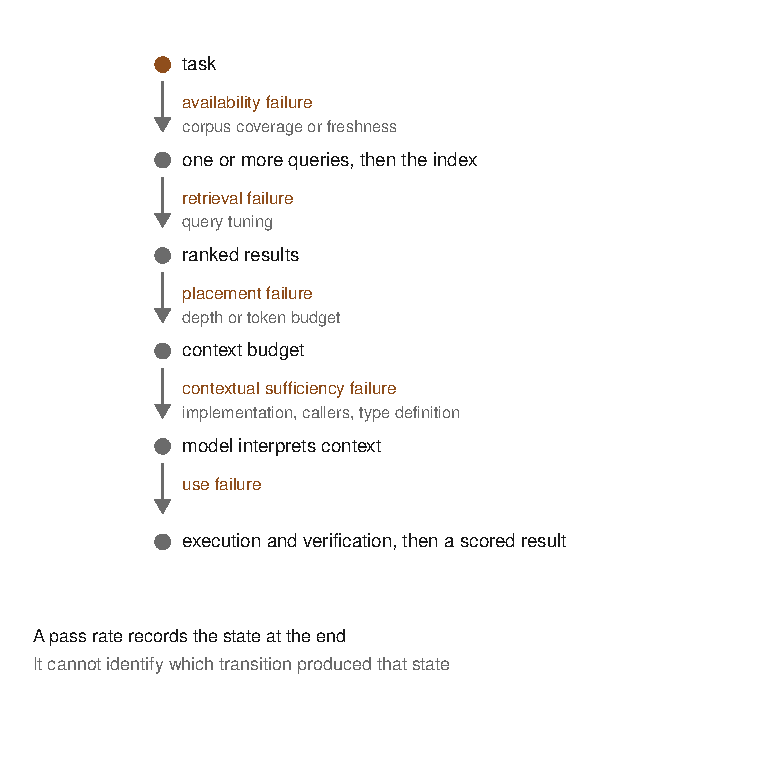
\includegraphics[keepaspectratio,alt={The retrieval chain separates availability, retrieval, placement, contextual sufficiency, and use failures across the transitions from task formulation to scored execution and verification.}]{figures/ch11-retrieval-chain.pdf}}
\caption{The retrieval chain separates availability, retrieval, placement, contextual sufficiency, and use failures across the transitions from task formulation to scored execution and verification.}
\end{figure}

Pass rate captures only the final state, so it cannot reveal which transition failed or which governing condition caused the result.

The same ambiguity appears when a task passes. A generator may solve a familiar edit from model knowledge while the retriever returns irrelevant material. A broad retriever may place the answer somewhere in a large dump that exceeds the model's useful attention and still receive credit, because the final edit happens to work. Chapter 6's return-everything case reached recall 1.0 by construction. Correctness at the end of the run does not certify the evidence path that preceded it.

I therefore keep a per-task record with at least four fields: the identifiers of the judged relevant items, their positions in the returned list, the subset that entered model context, and the final task outcome. When the system exposes citations, tool references, or another reliable evidence-use signal, I add which items the generator actually used. A copy of the retrieved text in the prompt establishes exposure alone.

Repository-level code completion research supplies a clean example of this decomposition. RepoBench, from Liu et al.~(\href{https://arxiv.org/abs/2306.03091}{2023}), evaluates retrieval, completion with supplied context, and the combined pipeline as separable conditions. This design distinguishes a system that cannot retrieve the useful cross-file context from one that receives that context and cannot complete the code. A better ranker addresses the first failure and leaves the second untouched.

Memory evaluations expose a similar split through different measurements. MemConflict, from Tao et al.~(\href{https://arxiv.org/abs/2605.20926}{2026}), combined final-answer scoring with observations of whether the required memory was absent, ranked too low, retrieved but unused, or used incorrectly. Its evaluated systems answered correctly while the best reported conflict-recognition score across them reached only 0.2501. Memory Circuit Analysis, from Mao et al.~(\href{https://arxiv.org/abs/2605.03354}{2026}), reports a stage-level diagnostic that localizes a silent failure to the memory operation responsible for it, because extraction, retention, and retrieval can fail behind fluent responses. These results support stage localization, but their memory workloads do not reproduce all of the constraints of repository-scale software work.

Three newer studies provide directional support for the same measurement shape. SkillEvolBench, from Lei et al.~(\href{https://arxiv.org/abs/2605.24117}{2026}), and EngramaBench, from Acuna (\href{https://arxiv.org/abs/2604.21229}{2026}), examined whether stored or evolved material remained available and useful while also reporting final answers. A cost-and-accuracy study by Wolff and Bennati (\href{https://arxiv.org/abs/2601.07978}{2026}) separated what a memory system retrieves from what the answering model produces. I use those three to establish direction, and not as a numerical basis for a repository retrieval policy.

\subsection{Retrieval metrics}\label{retrieval-metrics}

With one required item, the per-task \href{mailto:Recall@k}{\nolinkurl{Recall@k}} value is binary, because the item is either present or absent. With several required items, it is the fraction found in the first \(k\). The aggregate reports the mean across tasks. When tasks require unequal numbers of items, that mean and the pooled fraction over all required items are different estimands, and the report should name the one it uses. The relevance judgment must also state which items count.

A file-level version counts the needed file, while a chunk-level version can require the specific definition or surrounding block. Those targets answer different questions and must be named.

The \textbf{rank} of a needed item is its position in the ordered results, with position one returned first. An item at position one and an item at position ten both count as retrieved when \(k=10\), although the first consumes less context and is less vulnerable to truncation. A single \href{mailto:Recall@k}{\nolinkurl{Recall@k}} value does not record that difference. When several items are needed, I record each position or a stated aggregate, because one number rarely describes the set.

Retrieval depth is an experimental variable. I sweep \(k\) across a range and plot recall as a function of depth. The \textbf{recall plateau} is the region where that curve flattens. Past it, returning additional items recovers little more required evidence. Choosing \(k\) before inspecting the curve biases every comparison.

A shallow cutoff can make a viable retriever look incapable. A deep cutoff can conceal poor ranking, because a disordered list still contains the target somewhere among its returned items. The plateau does not determine the operating point on its own, since latency, context consumption, and distractors can justify stopping earlier. It shows what recall the ranking can reach and the marginal cost in returned items.

\begin{figure}
\centering
\pandocbounded{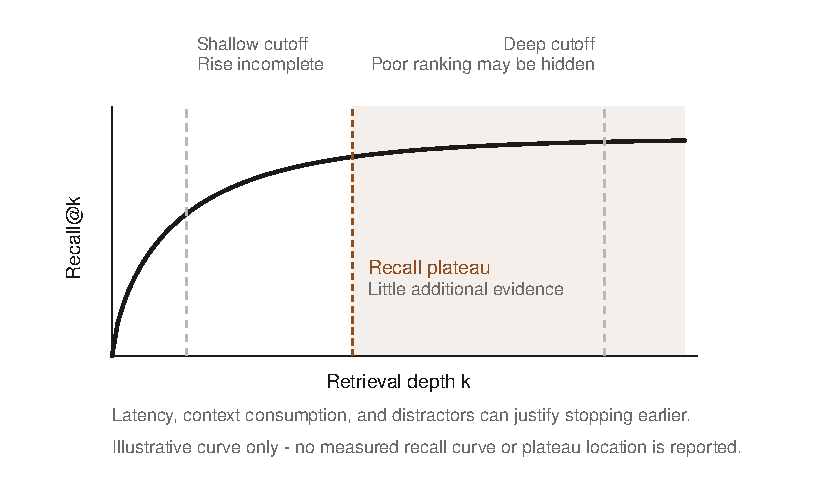
\includegraphics[keepaspectratio,alt={An unmeasured recall curve rises and plateaus with retrieval depth, but a shallow cutoff leaves gains unrealized, a deep cutoff can mask poor ranking, and latency, context use, or distractors may justify stopping earlier.}]{figures/ch11-recall-depth.pdf}}
\caption{An unmeasured recall curve rises and plateaus with retrieval depth, but a shallow cutoff leaves gains unrealized, a deep cutoff can mask poor ranking, and latency, context use, or distractors may justify stopping earlier.}
\end{figure}

Shallow cutoffs understate retrieval capability, while deep cutoffs can hide poor ranking. Latency, context consumption, and distractors may justify stopping before the plateau.

Multiple retrieval channels produce ordered lists whose numeric scores often have different meanings. BM25, a lexical ranking function based on term occurrence and document statistics, can emit values well above one. Cosine similarity for embedding vectors usually occupies a bounded interval. Adding or averaging those raw values gives arbitrary influence to whichever implementation happens to produce larger numbers.

\textbf{Reciprocal-rank fusion} combines lists by position. Each item receives a contribution such as \(1/(c+r)\) from each lane, where \(r\) is its position and \(c\) is a fixed damping constant. The fused order depends on agreement and placement across lists, and it ignores incomparable score scales.

Each of these measurements is incomplete in a different way. A single \href{mailto:Recall@10}{\nolinkurl{Recall@10}} can be useful, but it does not show whether ten sits before or after the plateau. A mean rank does not report the tasks in which the target did not appear at all. Missing items therefore need an explicit convention and a separate recall report. A fused list can improve coverage even when one channel has failed, and that failure is visible only when the original lane results remain available.

Stage-level evaluation requires relevance judgments. In a curated benchmark, maintainers can identify the file, symbol, span, or set of dependencies needed to solve each task. In a production repository, relevance may be plural and conditional. One correct patch may use the interface declaration and a caller. Another may use the implementation and a test. Declaring only one path relevant can penalize an equally valid evidence route.

I build judgments from the task's accepted solution, dependency structure, and expert review when the evaluation warrants that expense. I retain graded labels when an item can be useful without being sufficient. A class declaration may receive a relevance label, for example, while the concrete override receives a sufficiency label for the task. Whichever label schema is used, the record must document what qualified an item and which valid solution paths the annotators considered.

The expense limits where decomposition can be applied. Repository-scale relevance judgments require people who understand both the task and the codebase, and a changing repository can invalidate them. Sampling can control the cost. Annotate a stratified subset, preserve the adjudication record, and use it to diagnose the rest of the evaluation without pretending that unlabeled tasks have measured retrieval quality. A retrieval proxy based only on file overlap with one reference patch is cheaper, and it should be reported as that proxy.

Five terms can help reviewers describe the retrieved context: relevance, sufficiency, isolation, economy, and provenance. Relevance asks whether an item bears on the task. Sufficiency asks whether the returned set contains enough evidence to act correctly. Isolation asks whether the evidence is separated from material likely to mislead the model. Economy measures the context consumed to convey the evidence. Provenance records where the item came from and which version it represents.

This vocabulary comes from a position paper by Vishnyakova (\href{https://arxiv.org/abs/2603.09619}{2026}) and is not a measurement protocol. Each property needs an operational definition tied to the evaluated system before it can enter a score.

Evidence-use measurement is harder than exposure. Model-generated citations can be incomplete or post hoc. Removing one retrieved item and rerunning the task is an ablation, but model variability can change the output for reasons unrelated to that item. Attention weights do not establish causal use.

I therefore combine the available signals and state what each one supports. Exposure logs show what the model received. Citations show what it claimed to use. Controlled removal estimates whether the item changed outcomes across repeated runs.

The decomposition also changes the interpretation of verbose retrieval. Returning more material usually raises the chance that a relevant item appears, but it can reduce economy, isolation, and sometimes final performance. Precision and recall should therefore be reported together with context tokens and the completion score. A system that improves recall by filling the context window has made a different tradeoff from one that promotes the same evidence into its first few results.

Stage scoring is well established in benchmarked retrieval pipelines and much less established in end-to-end agent evaluation. Agents reformulate queries, inspect results, open additional files, and change direction as they work. One static top-\(k\) list does not represent that trajectory. I log each retrieval event with the query, lane, index version, results, positions, selection into context, and task state. The evaluation can then ask whether the needed evidence ever appeared, whether it appeared before the relevant decision, and whether a later query repaired an earlier miss.

This record supports engineering decisions the final score cannot. A missing indexed target, a low recall before the plateau, a good eventual recall with poor early ranks, and a relevant item excluded from context each point at a different stage. The categories are not perfectly independent, but they make the next ablation narrower and more informative.

\section{Recover the evidence a single lane misses}\label{recover-the-evidence-a-single-lane-misses}

My own literature-review pipeline ran for a period with its semantic search lane down while lexical search continued to return plausible results. Nothing in the completed reviews announced the missing channel. When I restored the lane and reran the searches, the combined search surfaced 64 additional papers across nine queries for one review and 42 across seven queries for another. Manual curation retained 12 and 7 of those papers.

The case illustrates a dangerous property of single-lane failure. The output remains coherent. A lexical query still returns documents that contain its terms. An operator therefore sees populated result lists rather than an outage, and the stack looks `healthy' from the outside. The absent papers became absent claims, qualifications, and related work in the downstream artifact. This case does not provide a general estimate of how many sources a semantic lane recovers. It shows why I keep lane health and lane contribution observable even when another lane appears to function.

The retrieval lane already present in a repository stack usually has a characteristic blind spot. Lexical systems rank on shared tokens. They are strong when a query contains a rare identifier, an exact error string, a configuration key, a function name, or the spelling used in code. They weaken when a task describes behavior in different language from the implementation. A request to ``stop duplicate jobs after a worker restart'' may depend on code named \texttt{claim\_epoch}, \texttt{lease\_owner}, or \texttt{dedupe\_key}, none of which occurs in the request.

CodeSearchNet, from Husain et al.~(\href{https://arxiv.org/abs/1909.09436}{2019}), framed this as a vocabulary gap between natural-language intent and source code. Repository agents face a wider version of the problem, because their queries mix prose, symbols, stack traces, and partial hypotheses. An embedding lane can connect semantically related text with little or no token overlap. It may retrieve a lease-recovery routine for the duplicate-job request even when the task does not use the routine's names.

The complement runs in the other direction. Embedding retrieval can place conceptually similar utilities near one another while missing the exact declaration that binds the edit. A query containing \texttt{ERR\_REPLAY\_DIVERGED}, a database column, or a generated type name often gives lexical search unusually discriminating evidence. Mapping those characters into a semantic neighborhood can discard the rarity that made the query useful.

The strongest code-specific case for keeping both lanes comes from an industrial study. Across 1,669 internal WeChat repositories and 26 language models, Yang et al.~(\href{https://arxiv.org/abs/2507.18515}{2025}) found that the combination of lexical and semantic retrieval performed best for closed-source code completion. The channels recovered complementary evidence rather than behaving as interchangeable implementations of one ranking function.

Those results do not establish the same ordering for every repository agent or for newer embedding models. The measured distribution was industrial, dominated by large C++ codebases and completion-style tasks. The design of the comparison transfers even when the result does not. Run each lane separately on the operated corpus and measure what each one uniquely recovers.

Production reports and late-interaction research support the same direction without settling it. A production account of agent memory (Trautmann 2026) describes parallel channels fused on ranks as a shipped default. Adaptive memory retrieval, from Yan et al.~(\href{https://arxiv.org/abs/2603.16496}{2026}), and late-interaction retrieval, from Khattab and Zaharia (\href{https://arxiv.org/abs/2004.12832}{2020}), support retaining a complementary semantic lane rather than any particular fusion policy. None of the three is code-specific evidence for the effect of fusion.

I run the channels separately and preserve their original lists. The lexical lane records its query, tokenizer, and index version. The semantic lane records the embedding model, vector index version, and filters. Per-lane \href{mailto:Recall@k}{\nolinkurl{Recall@k}} and target ranks show whether each lane contributes relevant items. The fused list is another stage, with its own recall, ranks, context consumption, and downstream completion score.

Rank fusion is necessary because channel scores have no shared unit. Suppose lexical search returns the exact symbol with a BM25 score of 18 and the semantic lane returns a conceptually related file with cosine similarity 0.84. The difference between 18 and 0.84 says nothing about relative relevance. Multiplying cosine similarity by 100 would reverse the implicit weighting without changing the semantic ranking at all. Any raw-score sum therefore embeds an arbitrary choice about scale.

Reciprocal-rank fusion discards that arbitrary magnitude and keeps ordinal evidence. An item ranked first by one lane and fifth by another receives support from both positions. An exact identifier hit ranked first lexically but absent semantically can still remain competitive. A broad conceptual match ranked moderately in both lanes can rise above results supported by only one channel. The damping constant controls how sharply the contribution falls with position, and it must be fixed and reported as part of the evaluated configuration. Selecting it after inspecting the completion scores turns it into the kind of researcher degree of freedom Chapter 1 describes.

Fusion does not establish that agreement means relevance. Two channels can share an ingestion error, retrieve the same stale version, or favor a heavily duplicated utility. Duplicated chunks can occupy several positions and create the appearance of independent support. I deduplicate stable item identities before or during fusion and retain provenance. Several representations of one source therefore do not count as independent support.

Filters also belong in the channel record. Restricting by language, repository area, branch, generated-code status, or modification time can improve isolation, but a wrong filter converts relevant evidence into an unreachable target. When the lexical and semantic lanes apply different filters, their apparent retrieval quality includes that policy difference. A useful comparison either holds the eligible corpus fixed or states that corpus selection is part of the lane under evaluation.

Semantic closeness is particularly hazardous when the corpus contains versions. An older implementation can be extremely close to the query and structurally similar to current code while prescribing an obsolete interface. Such a match becomes harmful when the generator selects it and acts on it, because it supplies a coherent but false basis for the edit. I record version and freshness with every result. The freshness gate in Chapter 12 can therefore reject evidence whose similarity exceeds its authority.

Each added lane also consumes resources. It adds index construction, storage, query latency, failure modes, and another source of distractors. Parallel execution can reduce wall-clock latency relative to sequential searches, but it does not remove compute or operational cost. A lane belongs in the stack when it recovers useful evidence on the operated workload or provides needed resilience.

Measured demand can be asymmetric. In one corpus served by my own systems, I observed 7,993 keyword calls and 2,449 semantic calls across site traffic and benchmark runs. Those counts do not measure answer quality, and they reflect the interfaces and users exposed in that system. They do show why replacing the lexical lane with a semantic one would have ignored most of the expressed demand, even though the semantic lane remained necessary for vocabulary gaps.

I evaluate the additional lane through a paired ablation. The same tasks run with the existing lane, with the added lane alone, and with fused results under the same retrieval and context budgets. The outcomes are paired by task. The analysis therefore works on the per-task differences rather than on two aggregate recalls. I sweep depth for each original list and for the fused list, because fusion can move the point where the recall curve flattens. The per-task analysis records which targets only the lexical lane found, which only the semantic lane found, which both found, and which neither could retrieve.

Identifier-heavy tasks deserve their own stratum. Aggregate recall can hide a fusion policy that helps prose queries while demoting exact symbols. I identify these tasks from task construction and repository artifacts before comparing lane outcomes. Error-string lookup, symbol navigation, configuration lookup, and natural-language behavior queries may require different mixtures. The strata should remain measurements of the workload, and a small result cannot justify hand-built routing rules.

The companion catalog includes more elaborate retrieval paths. They cover explicit recovery across lexical gaps, iterative re-querying when a draft exposes missing context, retrieval gates based on expected benefit, investment in whichever end of the retrieval-and-generation pipeline is limiting, and a cheap-first funnel followed by reranking. Each can be useful when a two-lane stack has a measured failure that calls for it. None repairs an unobserved channel outage or makes raw scores commensurate.

The operational test is whether fusion recovers relevant evidence that the current lane systematically misses, without consuming more context than the generator can use. I inspect the recovered items, their ranks, and the tasks they change. A lane that contributes only duplicates and stale neighbors has added cost without adding usable evidence, whatever its semantic sophistication.

\section{Preserve code structure inside the retrieval unit}\label{preserve-code-structure-inside-the-retrieval-unit}

Replacing fixed line windows with syntax-aware chunks raised \href{mailto:Recall@5}{\nolinkurl{Recall@5}} by 4.3 percentage points on RepoEval, a repository-level code retrieval-and-completion benchmark, in the cAST study from Zhang et al.~(\href{https://arxiv.org/abs/2506.15655}{2025}). The same study reported a 2.67-percentage-point \href{mailto:Pass@1}{\nolinkurl{Pass@1}} increase on SWE-bench generation across languages. These are modest changes in the full pipeline. They are large enough to examine at the chunking-policy layer, because the intervention changes neither the model nor the repository's underlying information.

The chunking policy determines which units a retriever can rank and which units a context builder can select. The index rarely stores an entire repository as one document. It divides files into spans, attaches identifiers and metadata, then represents each span for lexical or embedding search. That division creates the objects over which \href{mailto:Recall@k}{\nolinkurl{Recall@k}} is measured. A relevant function cannot rank as a coherent item when the chunker has split its signature, body, and surrounding contract into unrelated records.

Fixed windows choose boundaries by line or token count. They are simple, deterministic, and available for any text format. Their weakness follows directly from the absence of code structure in the boundary rule. A 100-line window can end after a function signature and place the body in the next chunk. Another window can combine the end of one class, three imports, and the start of an unrelated helper, because those lines happen to be adjacent.

Overlap softens boundary damage without removing it. Repeating twenty lines between windows may keep a short definition intact, while duplicating common imports, comments, and boilerplate across many indexed items. Long methods still split. The repeated spans can crowd retrieval results and distort fusion unless the system deduplicates them. Overlap reduces severed context at the cost of index size and result redundancy.

An abstract syntax tree, or AST, represents source code as nested syntactic constructs produced by a parser. A class node contains method nodes, a method contains statements and expressions, and a conditional contains its branches. Syntax-aware chunking uses those boundaries as constraints while still respecting a size budget. It does not assume that every tree node should become a retrievable document.

The implementation begins with a file-level tree and a maximum chunk size expressed in tokens or another measure tied to the context system. When a node fits, the chunker can retain it as a candidate unit. When it exceeds the limit, the chunker descends into its children and repeats the test. Small adjacent sibling nodes are merged while their combined representation remains within budget. The result tends to preserve complete functions, methods, classes, or coherent statement groups, and to avoid arbitrary line intervals.

Comments, decorators, attributes, and signatures require explicit attachment rules. A parser may represent them as siblings or metadata even though a reader treats them as part of the declaration that follows. Losing a decorator can erase authorization or routing behavior, and losing a leading comment can remove a constraint absent from the code. I test these attachments per language, because the generic tree shape may not capture the unit a programmer needs.

Imports and type definitions create another boundary decision. Copying all imports into every chunk increases local interpretability and token cost. Keeping imports only in a file header preserves the original structure but can leave a retrieved method with unresolved names. A practical design stores stable file and symbol metadata with every chunk and lets the context assembler retrieve a small companion span when a task requires import or type resolution. Sufficiency and economy determine the choice, but the tree alone does not.

The idea is language-general, but the parsing is not. Each supported language needs a parser that recognizes the repository's syntax version, including extensions, generated forms, and incomplete files. Parse failures need an explicit fallback, such as fixed windows with a failure flag. Silently dropping an unparseable file creates a corpus-coverage defect that can later look like a retriever miss.

Incremental indexing adds state. A changed file must be reparsed, old chunk identities retired, new chunks written, and references updated in an order that does not expose an empty or mixed version to queries. Stable identities based only on line offsets will churn when lines are inserted near the top of a file. Symbol-qualified identities can survive some edits, but overloaded or anonymous constructs still require versioned disambiguation. The index should record the source revision from which every chunk was derived.

Syntax is only a partial account of meaning. A large function can contain several responsibilities that deserve separate retrieval units, while a small method may be unintelligible without a protocol implemented across neighboring methods. Macros, reflection, generated bindings, configuration, and build files can carry semantics that a language AST does not express. Syntax boundaries preserve structural coherence, but they do not discover every semantic dependency.

The reported 4.3-percentage-point retrieval gain should be interpreted at that scale. It shows that chunk boundaries moved relevant code into the first five results on the studied tasks. It does not imply that structural chunking repairs a missing repository, a stale index, a query that names the wrong concept, or a retriever unsuited to code. A chunker can only shape items that enter the index, and only within the evidence the ranking system can recognize.

The 2.67-percentage-point generation gain is smaller and downstream. Improved retrieval has to survive context selection and then alter the model's completion. The difference between the two reported gains is consistent with the stage chain developed earlier, although the study alone does not identify a single cause for the attenuation. Some newly retrieved chunks may be redundant, some may enter below the usable cutoff, and some may fail to change generation.

I evaluate chunking policies on identical repository revisions and tasks. The fixed-window and syntax-aware indexes use the same eligible files, retrievers, queries, and top-\(k\) sweeps. Relevance judgments identify both the needed symbol and acceptable supporting neighbors. I then compare chunk recall, target rank, returned tokens, duplicate content, parse-failure coverage, and final completion.

Chunk recall needs a stated unit. When the target is a method, a chunk containing one line of that method should not count as fully relevant. The span must contain the task-specific evidence named in the judgment, such as the complete signature and the relevant branch, and partial matches should be reported separately when they help explain failures. File recall remains useful for diagnosing corpus and coarse retrieval, but it cannot certify that the returned chunk is interpretable.

Size deserves a sweep of its own. Very small syntax chunks improve isolation but can strip the relationships needed to understand state changes. Very large chunks preserve local structure while consuming the context budget and lowering the number of distinct candidates the model can inspect. I sweep the size budget together with retrieval depth, because those controls interact. Ten 200-token chunks and ten 1,500-token chunks impose different costs even when both are called \href{mailto:Recall@10}{\nolinkurl{Recall@10}}.

The implementation must also preserve ordering and provenance. When several chunks from one file enter context, their source order can help the model reconstruct control flow. Every chunk should name its file, symbol path, source revision, and line range for audit and follow-up retrieval. Those fields trace a failed completion back to the exact indexed representation.

Structural chunking is justified when the measured gain covers parser maintenance and indexing complexity for the supported languages. A repository dominated by languages with reliable parsers and long structured files is a strong candidate. A heterogeneous corpus containing templates, notebooks, generated fragments, and proprietary languages may need mixed policies. The correct unit follows the workload and the available structure.

The final comparison returns to decomposed scoring. I measure whether syntax-aware chunks recover the required evidence and where they rank, then whether those chunks improve completion under the same context budget. A better chunk recall with unchanged completion is still a diagnostic result. It says the chunker repaired its stage and that the remaining limit lies elsewhere in the path.

\section{Run the retrieval protocol on the operated workload}\label{run-the-retrieval-protocol-on-the-operated-workload}

Begin with the stack that serves real tasks. A reduced first version needs only a small sample from one query class, sized to the available annotation budget and stratified across the repositories or task shapes the decision depends on. Judge the needed evidence and instrument the stack already in production. A retrieval-depth sweep on that stratum can settle one decision: whether the production top-\(k\) cutoff should move for that query class.

For each task, identify the file, symbol, or evidence set that a competent solution can use. Log every retrieval query, the index revision, the returned item identities and ranks, which items enter model context, and the final task result. When direct evidence-use signals exist, preserve them without treating exposure as proof of use.

Compute file recall and chunk recall separately. Sweep retrieval depth, because a cutoff of ten is usually a tool default rather than a measured operating point. Plot the recall curve, mark where additional results recover little new evidence, and record the context tokens and latency at every depth. Select an operating point under the workload's context and cost constraints, then keep the full sweep with the result so another reader can see what the cutoff excluded.

Separate tasks by the evidence they demand. Exact symbols, error strings, natural-language behavior descriptions, cross-file dependencies, and version-sensitive questions exercise different retrieval paths. Preserve those strata before comparing systems. A gain concentrated in one query class can justify routing or a second lane even when its aggregate effect is small.

If the current stack has one lane, add the missing lexical or semantic lane as a controlled arm. Run each lane alone and retain their original rankings. Fuse positions, because the numeric scores are incommensurate. Measure which relevant items each lane uniquely recovers, which stale or duplicated items it adds, and how the fused list changes completion under a fixed context budget. Keep channel health visible in operation so a populated result list cannot conceal a lane outage.

Build a second index with syntax-boundary chunks when reliable parsers exist. Hold corpus eligibility, repository revision, query set, and retriever fixed. Sweep chunk size and retrieval depth together, and report parse failures and fallback coverage. Compare target ranks, recall, returned tokens, duplication, and completion against the existing chunker. The measured difference, including no difference, decides whether the parser and indexing complexity belong in that repository.

Read the resulting table by stage. Missing targets call for corpus or index work. Targets absent before the recall curve flattens call for a different query or retrieval lane. Targets found but ranked beyond the context cutoff call for ranking, fusion, or selection work.

Adequate evidence in context with an unchanged completion score shifts the next ablation downstream. Decomposition narrows the intervention without claiming that any one metric represents the whole system.

The retrieval depths, fusion constants, and chunk sizes in this chapter are not settings to adopt. Each is a parameter whose effect must be measured on the repository distribution, task mix, model, and context budget in use. Chapter 12 takes up the architecture around these measurements, including cheap retrieval funnels, typed indexes, and the conditions under which apparently relevant context should be refused as stale.

\section{Sources and evidence}\label{sources-and-evidence}

The evidence class and strength on each entry below come from its catalog record. Author-system cases in this chapter are narrative illustration and are not part of the evidence base.

\subsection{Score retrieval and generation separately}\label{score-retrieval-and-generation-separately-1}

\begin{itemize}
\tightlist
\item
  lit/strong: Liu, T., et al.~(2023), ``RepoBench: Benchmarking Repository-Level Code Auto-Completion Systems,'' ICLR 2024, arXiv:2306.03091. (R/C/P decomposition localizes failure to retrieval vs completion vs pipeline stage.)
\item
  explorer/strong: MemConflict (Tao et al.~2026), arXiv:2605.20926. (Black-box + white-box memory evaluation; localizes missing vs low-ranked vs retrieved-but-unused; best reported conflict-recognition score 0.2501.)
\item
  explorer/strong: Memory Circuit Analysis (Mao et al.~2026), arXiv:2605.03354. (Stage-level diagnostic localizing a silent failure to the responsible memory operation; extraction/retention/retrieval fail silently behind fluent answers.)
\item
  explorer/directional: SkillEvolBench (Lei 2026), arXiv:2605.24117. Direction only.
\item
  explorer/directional: EngramaBench (Acuna 2026), arXiv:2604.21229. Direction only.
\item
  explorer/directional: Cost-and-Accuracy study (Wolff \& Bennati 2026), arXiv:2601.07978. Direction only.
\item
  lit/anecdotal: Vishnyakova, O. (2026), arXiv:2603.09619. (Names the five context-quality criteria; position paper.)
\end{itemize}

\subsection{Hybrid retrieval fused on ranks}\label{hybrid-retrieval-fused-on-ranks}

\begin{itemize}
\tightlist
\item
  lit/strong: Yang, Z., et al.~(2025), ``A Deep Dive into Retrieval-Augmented Generation for Code Completion: Experience on WeChat,'' arXiv:2507.18515 (industrial study).
\item
  explorer/strong: CodeSearchNet vocabulary-gap framing (Husain 2019), arXiv:1909.09436. (Exact/lexical match as a first-class lane fused on ranks; score fusion broken by construction.)
\item
  explorer/directional: Cloudflare ``Agents that remember'' (Trautmann 2026), the production account carrying the shipped default of parallel channels fused with reciprocal-rank fusion. No canonical URL is on record for this item. Direction only.
\item
  explorer/directional: AdaMem (Yan et al.~2026), arXiv:2603.16496, carried in the same evidence record as the Cloudflare account. Its own retrieval route is semantic retrieval with conditional graph expansion rather than rank fusion, so it supports retaining a complementary semantic lane only. Direction only.
\item
  explorer/directional: ColBERT (Khattab and Zaharia 2020), arXiv:2004.12832. Direction only.
\end{itemize}

\subsection{Chunk on AST boundaries}\label{chunk-on-ast-boundaries}

\begin{itemize}
\tightlist
\item
  lit/strong: Zhang, Y., et al.~(2025), ``cAST: Enhancing Code Retrieval-Augmented Generation with Structural Chunking via Abstract Syntax Tree,'' arXiv:2506.15655.
\item
  Corroboration for this entry: none on record. The other two entries in this chapter carry dossier corroborations from the author's own systems, which are illustration rather than independent sources.
\end{itemize}
